%tag:000X
%label:"fig:roundingCorner"
%author:JeffHicks
%name:"rounding corner in Polterovich surgery"
%type:"figure"
%parent:thm_roundingCorner
%caption:"By rounding the corner, we can compare holomorphic triangles with holomorphic strips on the surgery."


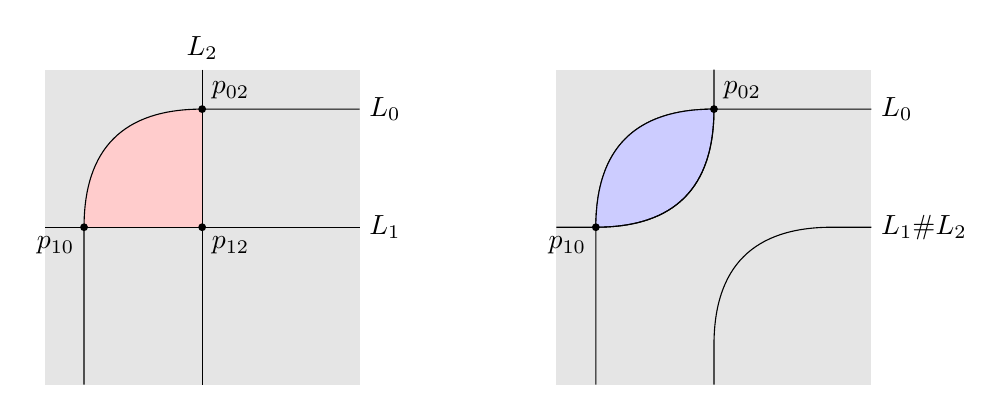
\begin{tikzpicture}\begin{scope}[]


    \fill[gray!20]  (-2,2) rectangle (2,-2);
    \fill[red!20] (0,0) .. controls (0,0.5) and (0,1) .. (0,1.5) .. controls (-1,1.5) and (-1.5,1) .. (-1.5,0) .. controls (1,0) and (0.5,0) .. (0,0);
    
    \draw (0, 2)--(0,-2);
    \draw (2,0) -- (-2,0);
    \draw (2,1.5) .. controls (1,1.5) and (0.5,1.5) .. (0,1.5) .. controls (-1,1.5) and (-1.5,1) .. (-1.5,0) .. controls (-1.5,-0.5) and (-1.5,-1.5) .. (-1.5,-2);
    
    \node[right] at (2,1.5) {$L_0$};
    \node[right] at (2,0) {$L_1$};
    \node[above] at (0,2) {$L_2$};
    \node[below right] at (0,0) {$p_{12}$};
\node[above right] at (0,1.5) {$p_{02}$};
\node[below left] at (-1.5,0) {$p_{10}$};
    \node[fill=black, circle, scale=.3] at (0,0) {};
    \node[fill=black, circle, scale=.3] at (0,1.5) {};
    \node[fill=black, circle, scale=.3] at (-1.5,0) {};
\end{scope}
    
    
    \begin{scope}[shift={(6.5,0)}]
    
    
    \fill[gray!20]  (-2,2) rectangle (2,-2);
    \draw (2,1.5) .. controls (1,1.5) and (0.5,1.5) .. (0,1.5) .. controls (-1,1.5) and (-1.5,1) .. (-1.5,0) .. controls (-1.5,-0.5) and (-1.5,-1.5) .. (-1.5,-2);
    
    \node[right] at (2,1.5) {$L_0$};
    \node[right] at (2,0) {$L_1\#L_2$};
    
    
    \draw[fill=blue!20] (0,1.5) .. controls (0,0.5) and (-0.5,0) .. (-1.5,0) .. controls (-1.5,1) and (-1,1.5) .. (0,1.5);
    
    \draw (0,2) .. controls (0,1.5) and (0,2) .. (0,1.5) .. controls (0,0.5) and (-0.5,0) .. (-1.5,0) .. controls (-2,0) and (-2,0) .. (-2,0);
    \draw (0,-2) .. controls (0,-2) and (0,-2) .. (0,-1.5) .. controls (0,-0.5) and (0.5,0) .. (1.5,0) .. controls (2,0) and (2,0) .. (2,0);
    
    
\node[above right] at (0,1.5) {$p_{02}$};
\node[below left] at (-1.5,0) {$p_{10}$};
    \node[fill=black, circle, scale=.3] at (0,1.5) {};
    \node[fill=black, circle, scale=.3] at (-1.5,0) {};
    \end{scope}
    
    \end{tikzpicture}%tag:000X
    %label:"fig:roundingCorner"
    %author:JeffHicks
    %name:"rounding corner in Polterovich surgery"
    %type:"figure"
    %parent:thm_roundingCorner
    %caption:"By rounding the corner, we can compare holomorphic triangles with holomorphic strips on the surgery."
    
    
    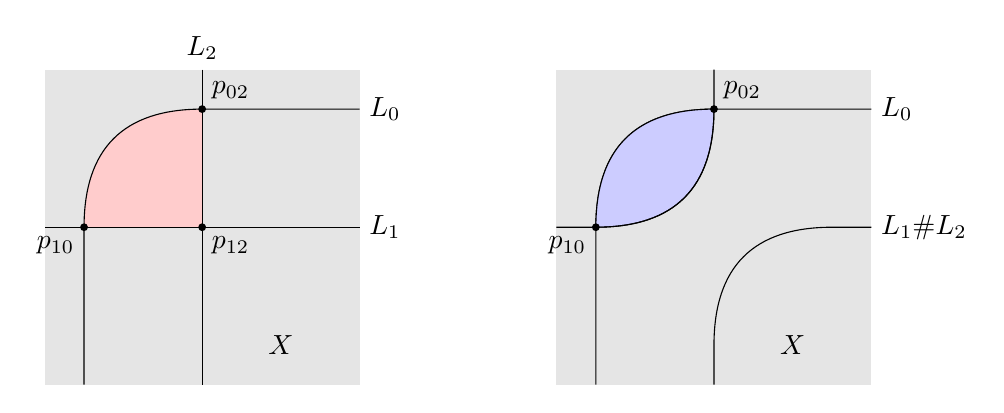
\begin{tikzpicture}\begin{scope}[]
    
    
        \fill[gray!20]  (-2,2) rectangle (2,-2);
        \fill[red!20] (0,0) .. controls (0,0.5) and (0,1) .. (0,1.5) .. controls (-1,1.5) and (-1.5,1) .. (-1.5,0) .. controls (1,0) and (0.5,0) .. (0,0);
        
        \draw (0, 2)--(0,-2);
        \draw (2,0) -- (-2,0);
        \draw (2,1.5) .. controls (1,1.5) and (0.5,1.5) .. (0,1.5) .. controls (-1,1.5) and (-1.5,1) .. (-1.5,0) .. controls (-1.5,-0.5) and (-1.5,-1.5) .. (-1.5,-2);
        
        \node[right] at (2,1.5) {$L_0$};
        \node[right] at (2,0) {$L_1$};
        \node[above] at (0,2) {$L_2$};
        \node[below right] at (0,0) {$p_{12}$};
    \node[above right] at (0,1.5) {$p_{02}$};
    \node[below left] at (-1.5,0) {$p_{10}$};
        \node[fill=black, circle, scale=.3] at (0,0) {};
        \node[fill=black, circle, scale=.3] at (0,1.5) {};
        \node[fill=black, circle, scale=.3] at (-1.5,0) {};
    \node at (1,-1.5) {$X$};
    \end{scope}
        
        
        \begin{scope}[shift={(6.5,0)}]
        
        
        \fill[gray!20]  (-2,2) rectangle (2,-2);
        \draw (2,1.5) .. controls (1,1.5) and (0.5,1.5) .. (0,1.5) .. controls (-1,1.5) and (-1.5,1) .. (-1.5,0) .. controls (-1.5,-0.5) and (-1.5,-1.5) .. (-1.5,-2);
        
        \node[right] at (2,1.5) {$L_0$};
        \node[right] at (2,0) {$L_1\#L_2$};
        
        
        \draw[fill=blue!20] (0,1.5) .. controls (0,0.5) and (-0.5,0) .. (-1.5,0) .. controls (-1.5,1) and (-1,1.5) .. (0,1.5);
        
        \draw (0,2) .. controls (0,1.5) and (0,2) .. (0,1.5) .. controls (0,0.5) and (-0.5,0) .. (-1.5,0) .. controls (-2,0) and (-2,0) .. (-2,0);
        \draw (0,-2) .. controls (0,-2) and (0,-2) .. (0,-1.5) .. controls (0,-0.5) and (0.5,0) .. (1.5,0) .. controls (2,0) and (2,0) .. (2,0);
        
        
    \node[above right] at (0,1.5) {$p_{02}$};
    \node[below left] at (-1.5,0) {$p_{10}$};
        \node[fill=black, circle, scale=.3] at (0,1.5) {};
        \node[fill=black, circle, scale=.3] at (-1.5,0) {};
    \node at (1,-1.5) {$X$};
        \end{scope}
        
        \end{tikzpicture}